%!TEX encoding = UTF-8 Unicode  
\documentclass{article}  
\usepackage{xeCJK}
\setCJKmainfont[BoldFont=STZhongsong, ItalicFont=STKaiti]{STSong}
\setCJKsansfont[BoldFont=STHeiti]{STXihei}
\setCJKmonofont{STFangsong}
\usepackage{graphicx}
\usepackage{amsmath}
 \usepackage{clrscode}
\usepackage{listings}
\usepackage{enumerate}
\lstset{language=C++}%这条命令可以让LaTeX排版时将C++键字突出显示

\lstset{breaklines}%这条命令可以让LaTeX自动将长的代码行换行排版

\lstset{extendedchars=false}%这一条命令可以解决代码跨页时,章节标题,页眉等汉字不显示的问题




\begin{document}  

\title{毕业论文}
\date{}

\maketitle


\textbf{中文摘要}关键词
      \qquad
\newline
\textbf{Abstract}Key words
      \qquad
\newline
\textbf{目录}
      \qquad
\newline

\textbf{一、引言}
      \qquad
\newline

\textbf{二、研究背景综述}
      \qquad
\newline

近年来,在工程应用中,求解高阶矩阵的需求日益增长,全矩阵运算脱离了实际的硬件限制,为了满足这一日益增长的需求,同时这些矩阵通常都有着一个特征——非零元远少于零元,稀疏矩阵这门学科便应运而生。
在 20 世纪 60 年代研发电子网络的电子工程师们是最早的去利用稀疏性来应用稀疏矩阵进行工程上的计算的。[1]
而在微分方程数值解、线性规划等的有限元分析中,经常出现求解高阶稀疏线性方程组,如利用全矩阵进行存储,则需要$n^2$的空间复杂度和$n^3$的乘法运算时间复杂度,显然,这种程度的运算量是无法被微型计算机,甚至是工作站所接受的。
而利用矩阵的稀疏性,可以有效地减小消耗很多无谓的存储空间以及无谓的计算,在很大的程度上降低了时间和空间复杂度,降低了计算对硬件的需求,使计算成为可能。
\newline
\textbf{(1)稀疏矩阵的定义}
      \qquad
\newline
稀疏矩阵是非零元远小于矩阵元素总数,且非零元分布没有规律的矩阵。[1]

\textbf{(2)稀疏矩阵已有存储方式}
      \qquad
\newline
在这些年的发展中,出现了很多的存储方法,比如:对角线存贮法、对称矩阵的变带宽存贮法、坐标存贮法、Elipack-Itpack存贮法、CSR存贮法、Shermans存贮法、超矩阵存贮法、动态存贮方案等[2]。
\newline
如行压缩存储方式(Compressed Row Storage):
CRS存储可以高效地存取任意一行非零元素,但存取任意一列非零元则需要遍历整个CRS存储结构。相应地,与CRS存储的稀疏矩阵相关的算法要高效的编程实现,算法的计算顺序必须按行来进行。[3]
下面对应于CRS存储:
\newline\newline\newline\newline\newline\newline\newline

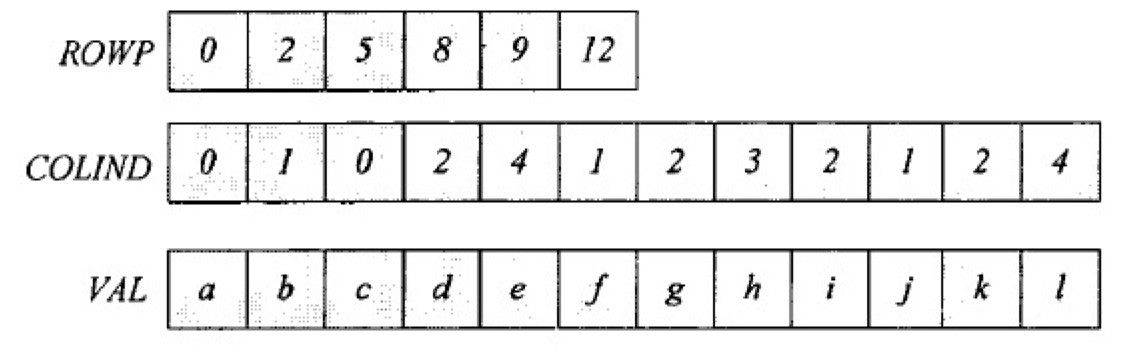
\includegraphics[scale=0.25]{crs.png}
我们可以发现,ROWP数组存储的时行非零元的增长量。COLIND则存储的是列索引值,典型的C语言结构实现为\newline

\begin{lstlisting}

struct cr_matrix{ 
	int *Ri;/*col index*/ 
	int *Rp;/*length nrow+1*/ 
	double *Rx; 
	int Rncol;
	int Rnrow;
};

\end{lstlisting}

\textbf{(3)已有的处理稀疏矩阵存储与运算的开源库}
      \qquad
\newline
在做稀疏矩阵的计算时,通常都是做一系列的基本运算,如:矩阵转置、矩阵向量乘法、矩阵矩阵乘法、数乘等。为了能得到更好的效率,许多研究者致力于寻找对于这些计算最优的存储结构及计算算法,同时提供了许多类库供科学计算使用,如:Portable, ExtensibleToolkit for Scientific Computation(PETSc)、Boost、GNU Scientific Library (GSL)等。\newline
例如,在Boost-uBLAS中有着稀疏矩阵的模板mapped\_matrix<T, F, A>(元素映射矩阵存储形式)、compressed\_matrix<T, F, IB, IA, TA>(压缩存储格式)、coordinat\_matrix<T, F, IB, IA, TA>(坐标存储格式)。
分别有着如下示例:[4]\newline
\textbf{mapped\_matrix:}
\begin{lstlisting}

#include <boost/numeric/ublas/matrix_sparse.hpp>
#include <boost/numeric/ublas/io.hpp>

int main () {
    using namespace boost::numeric::ublas;
    mapped_matrix<double> m (3, 3, 3 * 3);
    for (unsigned i = 0; i < m.size1 (); ++ i)
        for (unsigned j = 0; j < m.size2 (); ++ j)
            m (i, j) = 3 * i + j;
    std::cout << m << std::endl;
}

\end{lstlisting}

\textbf{compressed\_matrix:}
\begin{lstlisting}

#include <boost/numeric/ublas/matrix_sparse.hpp>
#include <boost/numeric/ublas/io.hpp>

int main () {
    using namespace boost::numeric::ublas;
    compressed_matrix<double> m (3, 3, 3 * 3);
    for (unsigned i = 0; i < m.size1 (); ++ i)
        for (unsigned j = 0; j < m.size2 (); ++ j)
            m (i, j) = 3 * i + j;
    std::cout << m << std::endl;
}

\end{lstlisting}

\textbf{coordinate\_matrix:}
\begin{lstlisting}

#include <boost/numeric/ublas/matrix_sparse.hpp>
#include <boost/numeric/ublas/io.hpp>

int main () {
    using namespace boost::numeric::ublas;
    coordinate_matrix<double> m (3, 3, 3 * 3);
    for (unsigned i = 0; i < m.size1 (); ++ i)
        for (unsigned j = 0; j < m.size2 (); ++ j)
            m (i, j) = 3 * i + j;
    std::cout << m << std::endl;
}
\end{lstlisting}



\textbf{三、研究的目标、内容及研究方法}
      \qquad
\newline
\textbf{(1)研究的目标}
      \qquad
\newline
利用c++在g++编译器linux平台下实现稀疏矩阵的行压缩存储方式(Compressed Row Storage)存储。可以并行计算稀疏矩阵的矩阵乘法、数乘等运算。
\newline

\textbf{(2)研究内容}
      \qquad
\newline
 在linux平台下,基于g++编译器,编写稀疏矩阵存储的C++库,实现稀疏矩阵的行压缩存储方式(Compressed Row Storage),同时实现一些稀疏矩阵的基本运算,如矩阵乘法、数乘等。为了更好地发挥CPU性能,需要实现多线程并行计算。

\textbf{(3)研究方法}
      \qquad
\newline
实现稀疏矩阵的行压缩存储方式(Compressed Row Storage),通过数组存储非零元的增长量、列索引值和非零元值来实现稀疏矩阵的存储。为了实现可变长数组的存储,利用C++的STL中的vector来存储数据。
\newline
而为了更好地利用CPU的性能,利用thread库实现多线程并行计算,更为有效地利用CPU的并行性能。而为了防止多线程并行计算中“脏数据”的出现,利用mutex互斥锁保障进程安全性。
\newline
为了实现稀疏矩阵的矩阵矩阵乘法和矩阵向量乘法,可以参考全矩阵矩阵矩阵乘法和矩阵向量乘法算法,利用稀疏矩阵的零元不参与计算的特性,按照稀疏矩阵存储的结构,较全矩阵计算省略大量计算,实现稀疏矩阵计算的优势——更为高效的计算。
\newline


\textbf{四、实验结果}
      \qquad
\newline









\textbf{五、结论}
      \qquad
\newline


\textbf{参考文献}
      \qquad
\newline
 [1]Yousef Saad.Iterative Methods for Sparse Linear Systems[M].SECOND EDITION.USA:Society for Industrial and Applied Mathematics,2003年.68.\newline
 [2]张永杰、孙秦.稀疏矩阵存储技术[J].长春理工大学学报,2006年,03期:38-41.\newline
 [3]冯广祥. 大型稀疏矩阵直接求解算法的研究及实现[8].  东北大学:系统工程,2010.\newline
 [4]Joerg Walter and Mathias Koch.Boost 1.57.0 Library Documentation-uBLAS. http://www.boost.org/doc/libs/1\_57\_0/libs/numeric/ublas/doc/index.html, 2011\newline

  \end{document}  
